\documentclass[12pt]{article}
\usepackage{graphicx}
\usepackage {color}
\usepackage{pdfpages}
\usepackage{float}
\usepackage{changebar}
\usepackage{enumitem,amssymb}
\renewcommand{\familydefault}{\sfdefault}
\usepackage[margin=1.2in]{geometry}
\usepackage{graphicx}
\usepackage{wrapfig}
\usepackage[super]{cite}
\usepackage{subcaption}
\usepackage[table]{xcolor}
\usepackage{amsmath}
\usepackage[sort, numbers]{natbib}
\usepackage{multirow}

%%%%%%%%%%%%Defining the margins %%%%%%%%%%%%%%%%%%%%%
\textheight 9.in
\textwidth 6.5in
\topmargin -.5in
\oddsidemargin 0in
\setlength{\parskip}{\smallskipamount}

%%%%%%%%%%%%%%Specific Commands %%%%%%%%%%%%%%%%%%
\newcommand{\eg}{{\em e.g.,}}
\newcommand{\ie}{{\em i.e.,}}
\newcommand{\etc}{{\em etc.,}}
\newcommand{\etal}{{\em et al.}}
\newcommand{\degrees}{{$^{\circ}$}}
\newcommand{\fig}[1]{\textbf{Figure #1}}

%%%%%%%%%%%%%%%%%%%%%%%%%%%% Setting to control figure placement
% These determine the rules used to place floating objects like figures 
% They are only guides, but read the manual to see the effect of each.
\renewcommand{\topfraction}{.9}
\renewcommand{\bottomfraction}{.9}
\renewcommand{\textfraction}{.1}
\renewcommand{\familydefault}{\sfdefault} %setting the san serif font

%%%%%%%%%%%%%%%%%%%%%%%% Line spacing
% Use the following command for ``double'' spacing
%\setlength{\baselineskip}{1.2\baselineskip}
% and this one for an acceptable NIH spacing of 6lpi based on 11pt
%\setlength{\baselineskip}{.9\baselineskip}
% The baselineskip does not appear to work when we include a maketitle
% command in the main file.  Something there must set the line spacing
% If we use this next command, then things seem to work.
\renewcommand{\baselinestretch}{.9}

\setcounter{secnumdepth}{0} %make no numbers but have a table of contents


\begin{document}

\title{Homework 1, Cardiac Action Potential Simulation}
\author{Jake Bergquist, u6010393}
\maketitle
\tableofcontents
\newpage

\section{Introduction}
\par{}
The purpose of this homework is to investigate the Ruo-Ludy 1994 model of a cardiac action potential. To that end I first ran the simulation with the prescribed default physiological parameters. From this simulation I plotted the resulting action potential at the membrane, the currents of IK1, IK, slow calcium ICa, IKp, and background current Ib. I then investigated changes in the action potential and these currents based on changes in different parameters of the model. I explored different strength and duration of stimulus combinations to examine the strength duration curve of this action potential. I then looked at changes to the action potential resulting from changes in extracellular sodium concentrations. I then considered the pathalogical conditions present during ischemia. During cardiac ischemia, extracellular potassium concentration increases. This results in changes to the currents of the action potential as well as the resting membrane potential. I hypothesise that as the external potassium concentration increases the resting emmbrane potential will also increase. This should reduce the ability of the sodium channels to de-inactivate. This should result in reduced excitability of the modeled cell. 

\section{Methods}
\par{}
Initially I ran the simulation based the default parameters using the built run Map script. From this the currents and action potentials were plotted. Then, in order to investigate the durations and strength of stimulus required to initiate an action potential with this model. To that end I wrote a script to run the simulation with stimulus durations between 0.5 seconds to 5 seconds at intervals of 0.05 seconds and stimulus strengths of -5 uA/cm\^2 to -55 uA/cm\^2 at intervals of 0.5 uA/cm\^2. This resulted in 9,191 simulations. For each of the durations I then selected the minimum stimulus strength that produced an action potential (as measured by a membrane voltage above 0 mV). I also selected representative action potentials to display from these simulations.
\par{}
For the investigation of modulating the external sodium concentration I ran simulations with external sodium concentrations ranging from 1 to 200 mM/L in intervals of 1 mM/L. This resulted in 200 simulations. For each simulation the action potentials were plotted and compared. Specific cases were identified and investigated.

\par{}
For the investigation of modulating the external potassium concentration I ran the sumulatio with external potassium concentrations ranging from 1 to 100 mM/L in intervals of 1 mM/L. This resulted in 100 simulations. For each simulation the action potentials were plotted and compared. Specific cases were identified and investigated.
\section{Results}

\par{}
As can be seen in Figure~\ref{fig:Initial} the model produces the expected currents under normal circumstances and a characteristic cardiac action potential. There is a large inward sodium spike initially as well as a IK1 (potassium inward rectifying) inward spike. During the investigation of the strength duration curve I performed 9,191 simulations with different stimulus strengths and durations. The resulting 9,191 action potentials are shown in Figure~\ref{fig:AllStrDurAP}. As there are too many to particularly enumerate, they are colored simply to make them distinguishable. As can be seen, some strength duration calculations did not poduce anything more than a transient depolarization (seen as the triangle between 0 and 100 s, under -50 mV). The remaining combinations resulted in soe form of action potential. Increased strengths and durations resulted in higher peak voltages. In particular higher peaks resulted from increased strength, and delayed peaks resulted from increased duration. These also affect the small drop pre-plateau. As can be seen there were some combinations that resulted in very minimal action potentials. There is however a distinct different between action potential producing combinations and non-action potential producing combinations. These results are summarized in Figure~\ref{fig:StrDur}. The strength axis is inverted for viewing. The line shown by the red dots and fit by the red polynomial is the strength duration curve, the combinations that just barely result in an action potential. We can see that this curve exhibits asymptotic behavior on both strength and duration axis.


\begin{figure}[H]
	
	\centering	
	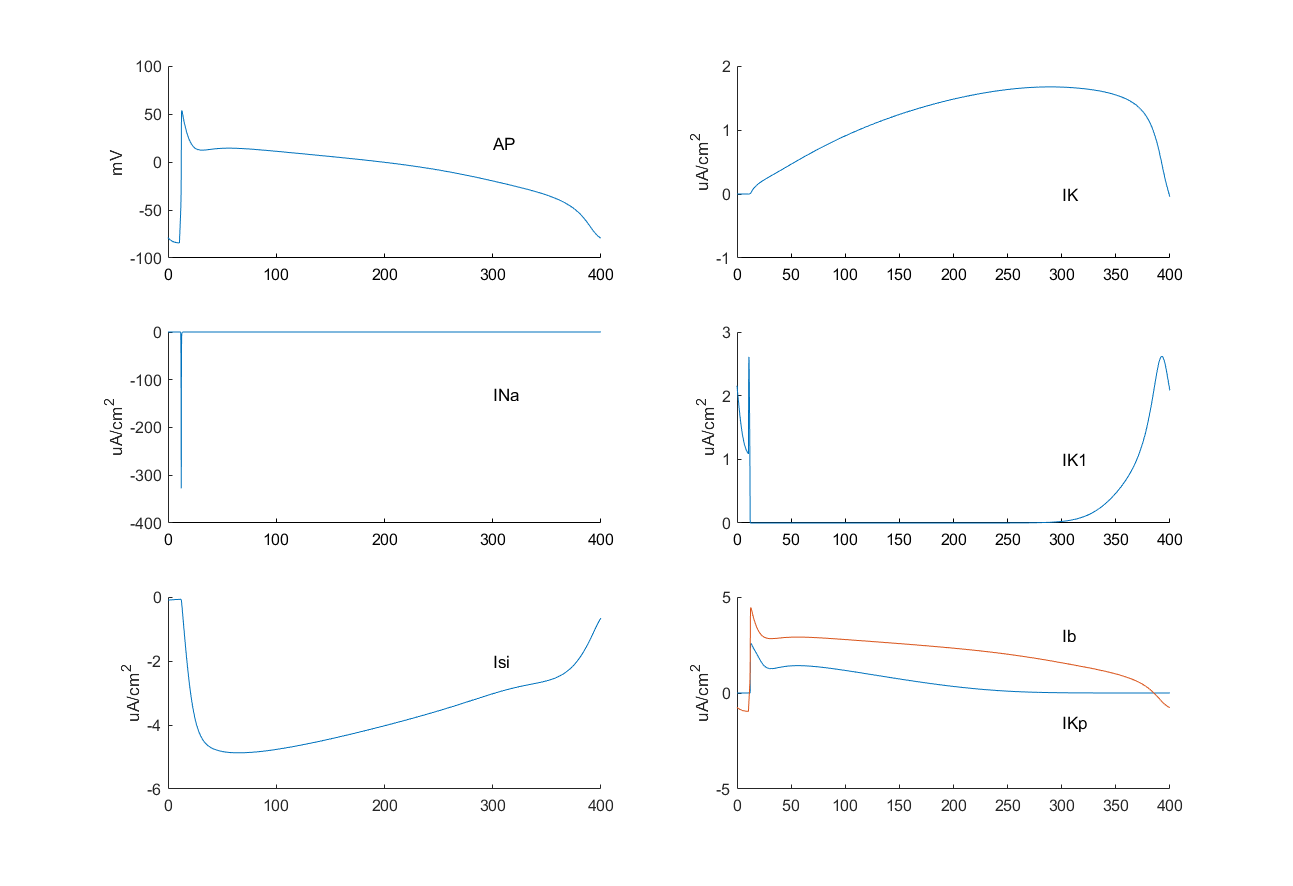
\includegraphics[width = 1\textwidth]{baseResults.png}
	\caption{ Results from the initial simulation with baseline parameters. Action potential and currents shown. X axis is in seconds. }
	\label{fig:Initial}
\end{figure}

\begin{figure}[H]
	
	\centering	
	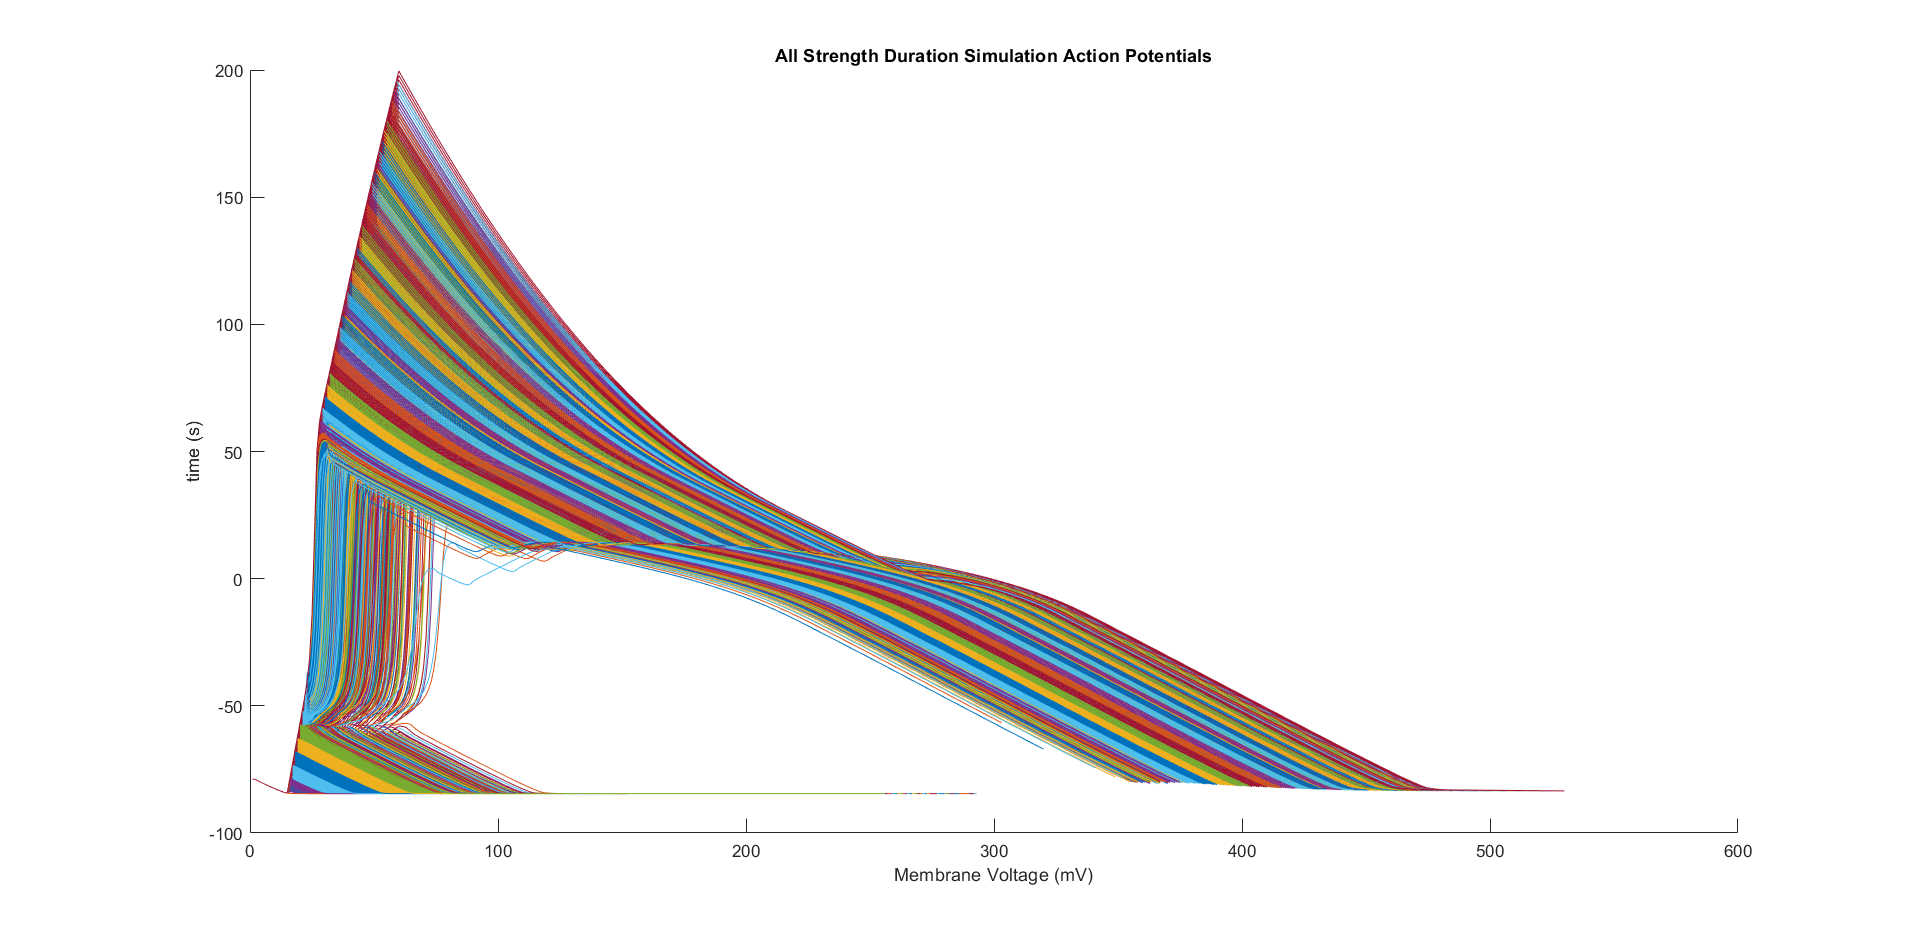
\includegraphics[width = 1\textwidth]{AllSimAP.png}
	\caption{ Results from the initial simulation with baseline parameters. Action potential and currents shown. X axis is in seconds. }
	\label{fig:AllStrDurAP}
\end{figure}

\begin{figure}[H]
	
	\centering	
	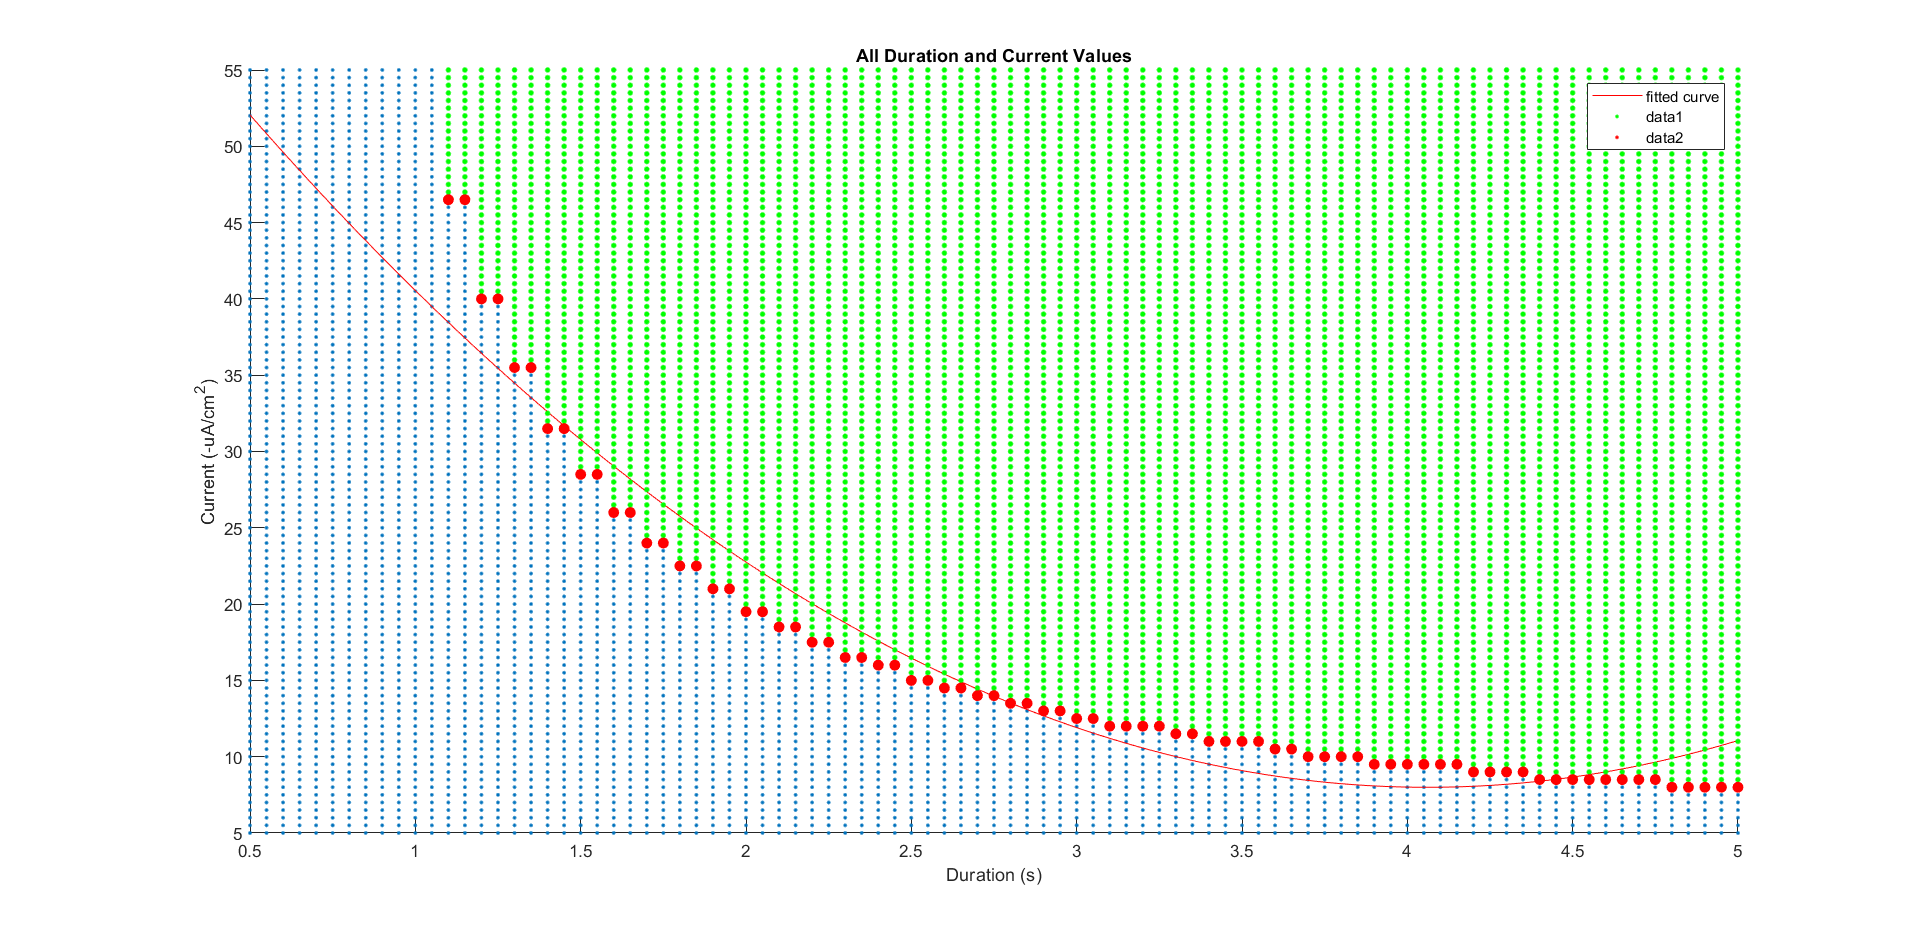
\includegraphics[width = 1\textwidth]{StrengthDuration.png}
	\caption{ Results the strength duration investigation. X axis is duration (seconds) and Y axis is strength (uA/cm\^2). Each dot is a strength duration combination. Blue dots are combinations unable to initiate an action potential. Green and Red dots are combinations that produced action potentials. Red dots are combinations with minimum strength for each duration, the ideal strength duration curve. The line is a polynomial fit to the ideal strength duration curve.  }
	\label{fig:StrDur}
\end{figure}

\begin{figure}[H]
	
	\centering	
	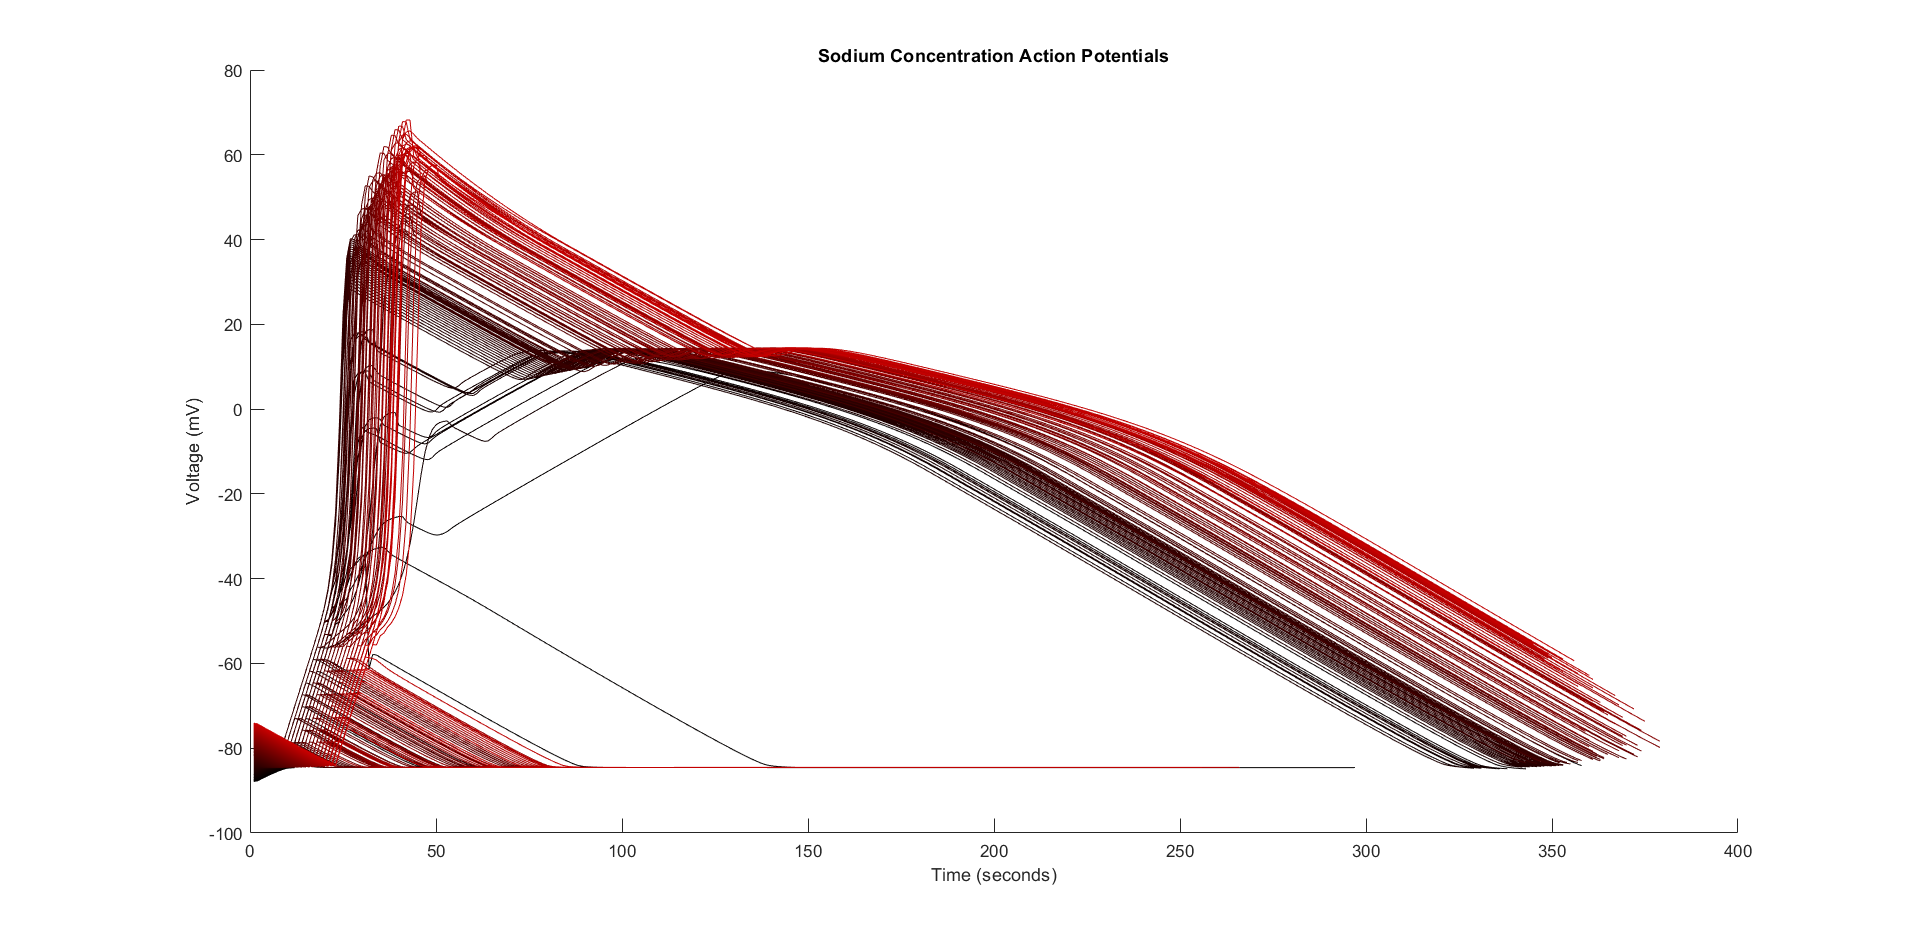
\includegraphics[width = 1\textwidth]{NaAPs.png}
	\caption{ Results from the Sodium concentration manipulations. More black action potentials are with low extracellular Sodium and more red with higher extracellular Sodium. The sodium concentration ranges from 1 mM/L to 200 mM/L. }
	\label{fig:AllNaAP}
\end{figure}

\par{}
As can be seen in Figure~\ref{fig:AllNaAP} variations in the Sodium concentration result in varied morphology in action potentials. As the extracellular Sodium rises from 1 uM/L to 200 uM/L the action potentials go from not firing at all, to having strange morphology. As the concentration approaches physiological levels the action potentials return to normal. Then as concentrations rise past physiological levels the action potentials increase in amplitude to an extent, then begin to not fire. It was of interest to investigate what happens when the concentration gradient approaches zero. To that end, I selected the situation where the gradient was zero (Figure~\ref{fig:NaCase}). As such I plotted the ionic currents at this gradient.

\begin{figure}[H]
	
	\centering	
	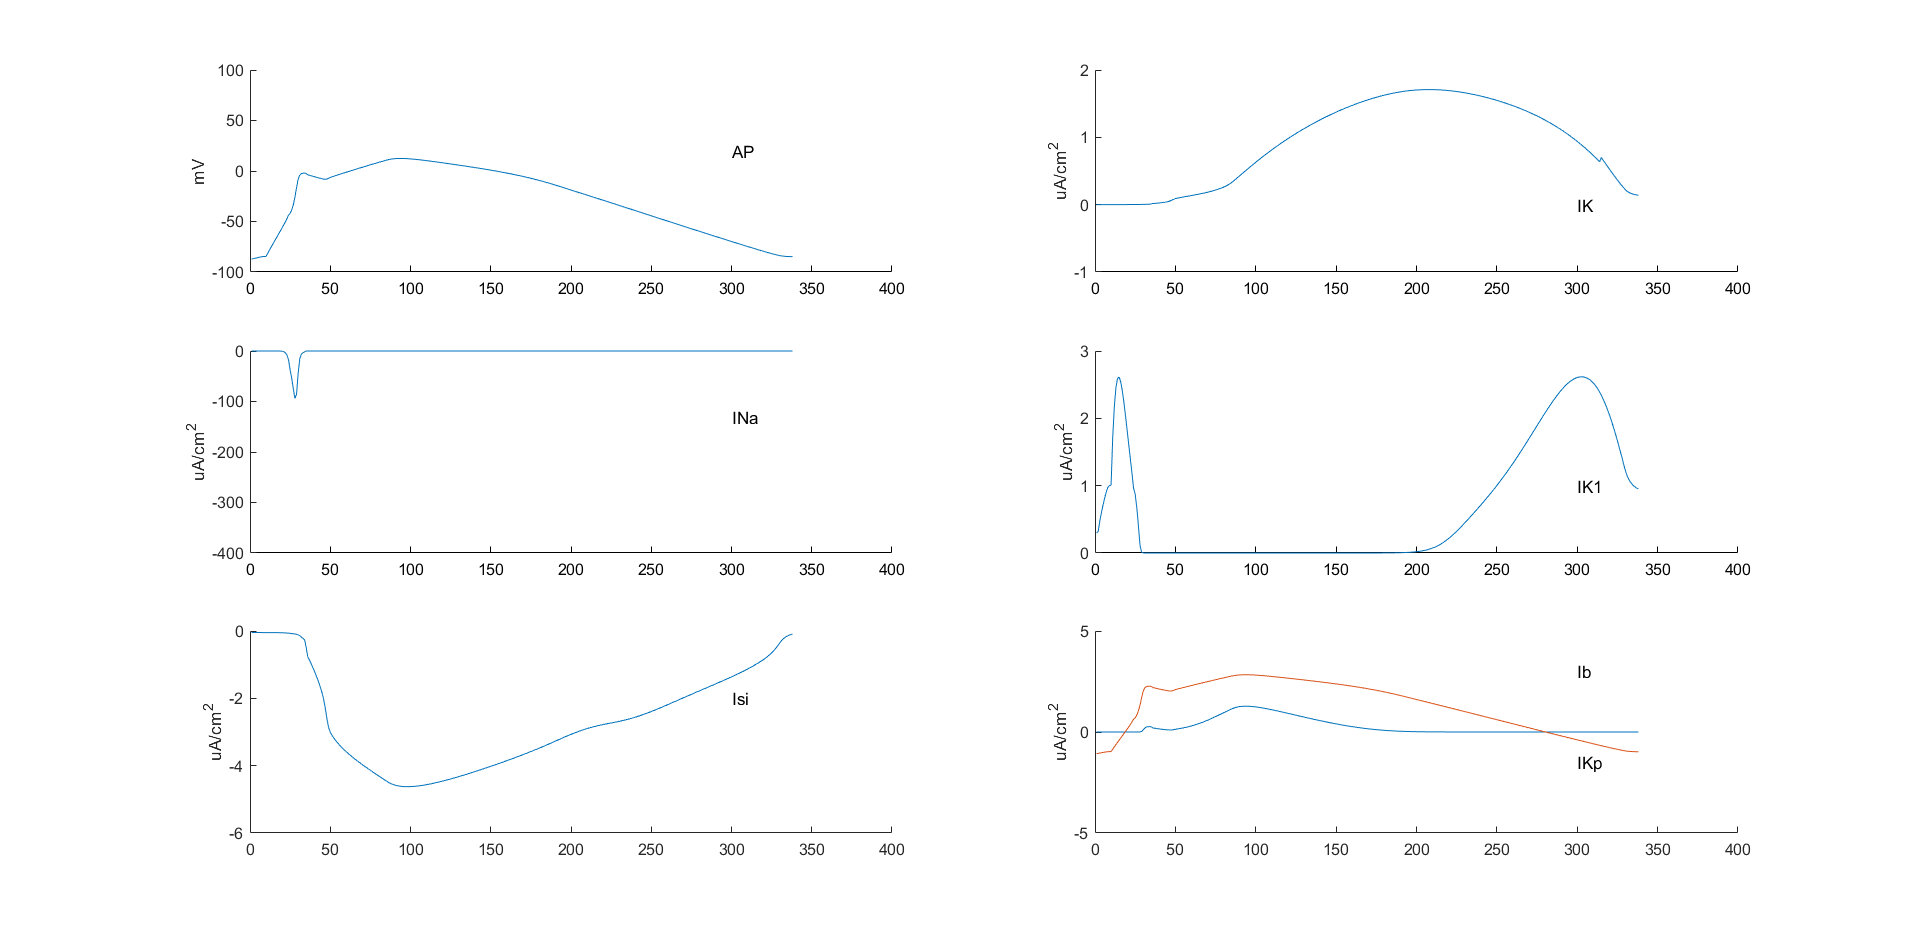
\includegraphics[width = 1\textwidth]{NaCase.png}
	\caption{ Results from the Sodium External Concentration at 10 mM/L. Action potential and all currents plotted. X axis in seconds. }
	\label{fig:NaCase}
\end{figure}

\par{}
I then chose to investigate changes in extracellular potassium, as are present in disease states such as Ischemia. At low extracellular potassium the action potentials do not fire. As this level rises the action potential fires earlier and earlier, the resting membrane value increases, and the peak of the action potential is reduced. As the concentration increases further the action potential ceases, and transient increases in membrane voltage are seen just due to stimulations.

\begin{figure}[H]
	
	\centering	
	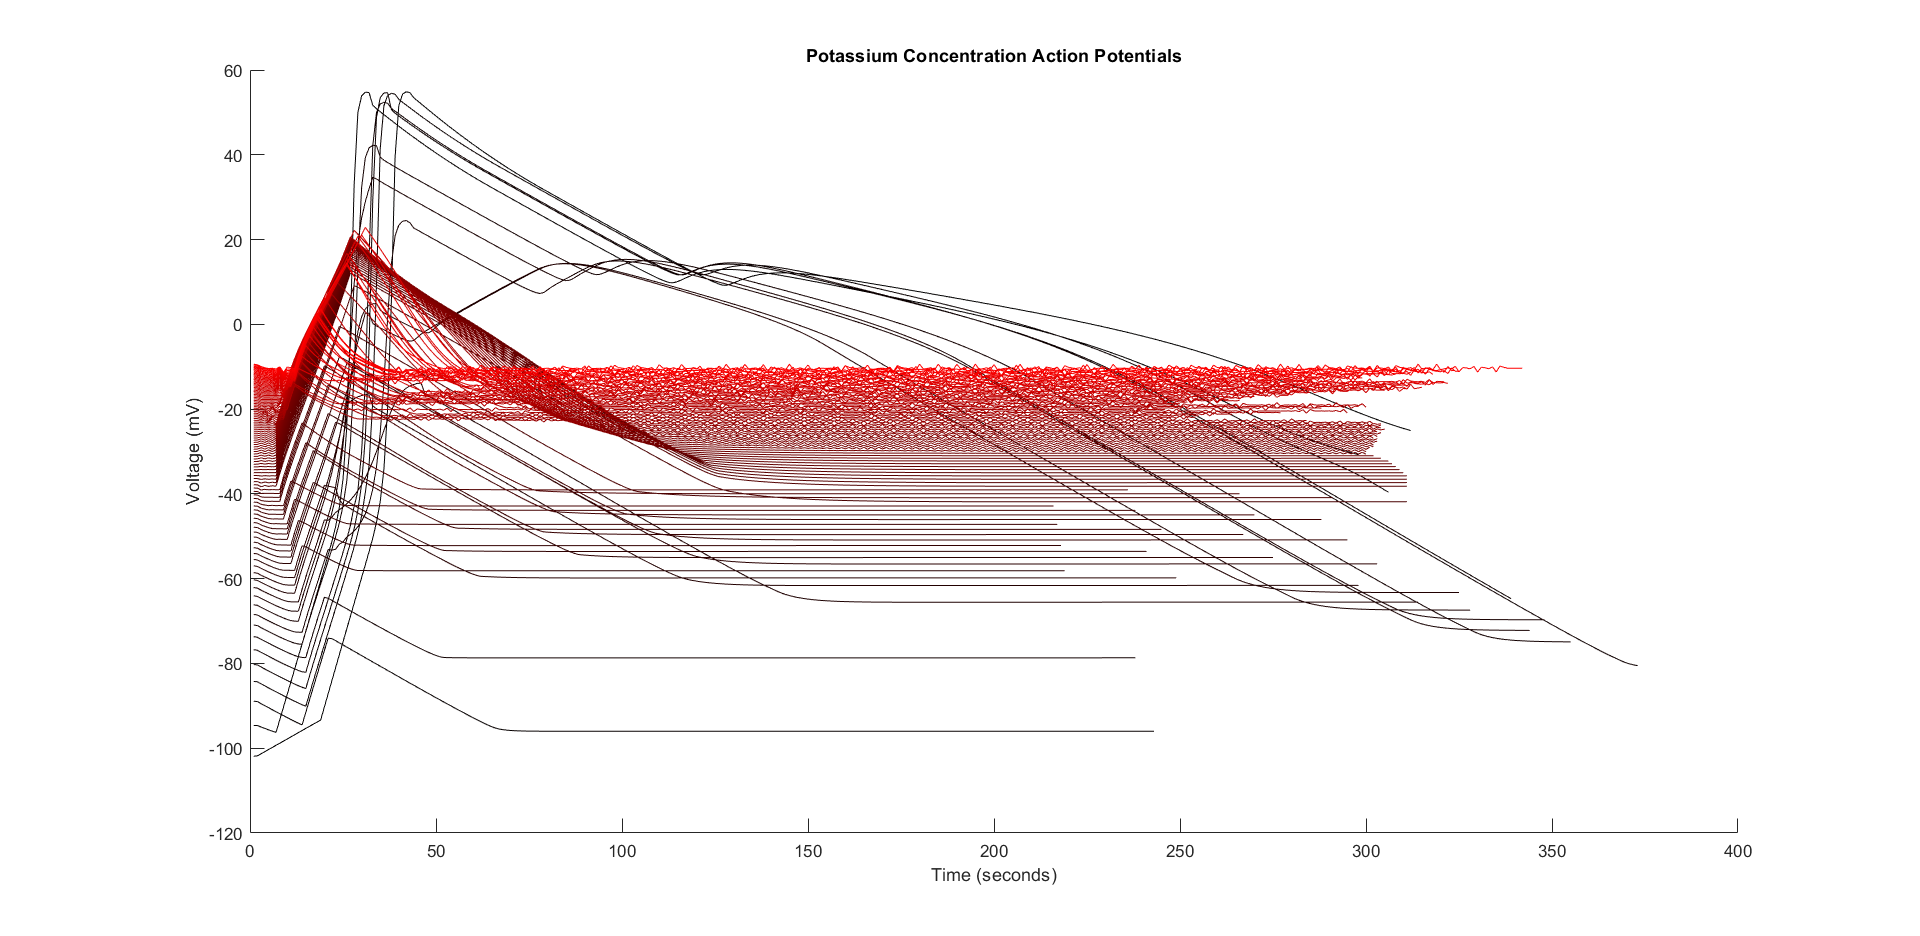
\includegraphics[width = 1\textwidth]{KAPs.png}
	\caption{ Results from the Potassium concentration manipulations. More black action potentials are with low extracellular Potassium and more red with higher extracellular Potassium. The Potassium concentration ranges from 1 mM/L to 100 mM/L. }
	\label{fig:AllKAP}
\end{figure}

\section{Discussion}
\subsection{1.a}
\par{}
Results shown above.
\subsection{1.b}
\par{}
As can be seen in Figure~\ref{fig:AllStrDurAP} there is a starg gap between combinations of strength and duration that can and those that cannot illicit an action potential. As such there is a threshold that the membrane voltage must reach before the action potential can fire, and before that point no action potential is possible (excluding anode break situations). Only strength and duration combinations that deliver enough charge to illicit such a depolarization result in action potentials. This demonstrates the all or nothing behavior of a n action potential. It either fires or it does not, no middle ground. Even the ones that barely fire, while their morphology may not be exactly a trypical action potential, they still fire.

\subsection{1.c}
\par{}
Results shown above.

\subsection{1.d}
\par{}
I attempted plynomial fitting as seen in Figure~\ref{fig:StrDur}. However a more apt fit would be a logorithmic fit. In either case the formula for determining if a certain strength and duration combination will result in an action potential alludes to the Rheobase and chronaxie. The Rheobase is the minimum strength needed to stimulate an action potential given an infinite duration. This is the duration asymptote of the curve characterized by the red dots in Figure~\ref{fig:StrDur}, roughly 5 uA/cm\^2. Double this strength is the chonaxie, which relates to the minimum energy needed in the system to reliably induce an action potential. Understanding this is critical for designing long lasting effective pacemakers.

\subsection{2}
\par{}
As the sodium concentration approached the point where the gradient was decreased the morphology of the action potential either changed or the action potential dropped out all together. However at a gradient of 0, where the extracellular and intracellular sodium concentrations were 10 mM/L there was still an action potential (Figure~\ref{fig:NaCase}). The cause of this is likely from the inwar rectifying potassium current driving the action potential, and a slight sodium current. The voltage gradient across the cell results in sodium still flowing inwards despite 0 concentration gradient. Additionally the large inward rectifying potassium (IK1) results in an abnormal, but still action potential peak. The remaining functioning currents behave normally to cause a plateau and repolarization as normal.
\par{}
Additionally when the extracellular sodium concentration becomes too high the action potential falls off. The model may not be well characterized in this space of very high external sodium concentrations. I am not sure why sometimes at high concentrations of extracellular sodium, no sodium current flows. However in these cases there is also abnormal IK1 current, potentially leading to a membrane voltage that does not reach threshold.

\subsection{3}
\par{}
During cardiac ischemia, extracellular potassium concentrations increase. This results in an increase in resting membrane potential. At first glance one would think this would result in more excitable cells as the membrane potential is closer to threshold, and at first this is true. However, in order to fire an action potential effectively, the sodium channels must be ready to open. When a sodium channel opens, it is eventually inactivated in a time dependent manner. The de-inactivation of the sodium channels can only occur effectively at low membrane voltages. If these channels cannot inactivate, they cannot open again to allow sodium current to initiate the next action potential. In this way, increased extracellular sodium can eventually prevent action potentials from firing. I hypothesized that I would see this behavior based on my understanding in the model. This phenomena was seen in the model (Figure~\ref{fig:AllKAP}). As the potassium concentration increased, so did the resting membrane potential. This resulted in early action potentials, as the membrane was closer to threshold, but a decreased amplitude of the peak, as more sodium channels were inactivated due to the higher membrane voltage. This continued until no acton potential was seen at all. At low potassium levels there also was no action potential. This is because there was no inward rectifying current to assist in the initiation of the action potential.


%%%%%%%%%%%%%%%%%% Correct Bibliography Style

\end{document}








